\scanpage{4}
\diagram{\begin{tikzcd}[ampersand replacement=\&,column sep=large,row sep=large]
A\times A \arrow[d,"\pi"'] \arrow[dr,phantom,"\text{\textcircled{cart}}"] \& A\times_S A\times_S B \arrow[l,"\operatorname{pr}_{12}"'] \arrow[d,"\pi\times\operatorname{id}_B"] \arrow[dr,"\operatorname{pr}_3"] \& \\
A \& A\times_S B \arrow[l,"\operatorname{pr}_1"] \arrow[r,dash,"\operatorname{pr}_2"'] \& B
\end{tikzcd}}
\diagram{\begin{tikzcd}[ampersand replacement=\&,column sep=large,row sep=large]
\& A\times_S A\times_S B \arrow[r,"\operatorname{pr}_3"] \arrow[d,"\operatorname{id}_{A\times A}\times\Delta_B=f"'] \arrow[ddl,bend right=45,"\operatorname{pr}_{12}"'] \arrow[dr,phantom,"\text{\textcircled{cart}}"] \& B \arrow[d,"\Delta_B"] \\
\& A\times_S A\times_S B\times_S B \arrow[r,"\operatorname{pr}'_{34}"'] \arrow[dl,dash,"\operatorname{pr}'_{12}"] \& B\times_S B \\
A\times_S A \& \&
\end{tikzcd}}
\[
\begin{aligned}
\Phi(F\overset{\mathbf L}{*}G)
&\overset{\mathrm{déf}}{\simeq}
\deleted{\mathbf R\operatorname{pr}_{2*}\bigl(\unsure{\mathbf L\operatorname{pr}_1^*(F\overset{\mathbf L}{\otimes}G)|\mathbf Lf^*(F\overset{\mathbf L}{\otimes}G)}\otimes\mathcal L\bigr)}\\
&\inserted{\mathbf R\operatorname{pr}_{2*}\bigl(\mathbf L\operatorname{pr}_1^*(F\overset{\mathbf L}{*}G)\otimes\mathcal L\bigr).}\\
&=\mathbf R\operatorname{pr}_{2*}\bigl(\mathbf L\operatorname{pr}_1^*(\unsure{\pi_*|\mathbf R\pi_*}(F\overset{\mathbf L}{\otimes}G))\inserted{\otimes\mathcal L}\bigr)\\
&\overset{\text{chgt. de base}}{\simeq}
\mathbf R\operatorname{pr}_{2*}\bigl(\mathbf R(\pi\times\operatorname{id}_B)_*\bigl(\mathbf L\operatorname{pr}_{12}^*(F\overset{\mathbf L}{\otimes}_S G)\bigr)\otimes\mathcal L\bigr)\\
&\overset{\text{formule de proj.}}{\simeq}
\mathbf R\operatorname{pr}_{2*}\bigl(\mathbf R(\pi\times\operatorname{id}_B)_*\bigl(\mathbf L\operatorname{pr}_{12}^*(F\overset{\mathbf L}{\otimes}_S G)\otimes(\pi\times\operatorname{id}_B)^*(\mathcal L)\bigr)\bigr)\\
&\overset{\text{transit.}}{\simeq}
\mathbf R\operatorname{pr}_{3*}\bigl(\mathbf L\operatorname{pr}_{12}^*(F\overset{\mathbf L}{\otimes}_S G)\otimes(\pi\times\operatorname{id}_B)^*(\mathcal L)\bigr).
\end{aligned}
\]
On a (th. du carré) un isom. can.
\[
(\pi\times\operatorname{id}_B)^*(\mathcal L)\simeq\operatorname{pr}_{13}^*(\mathcal L)\operatorname{pr}_{\unsure{13|23}}^*(\mathcal L)
\]
où $\operatorname{pr}_{13},\operatorname{pr}_{23}:A\times A\times B\mathbin{-}A\times B$ sont respectivement $\operatorname{pr}_1\times\operatorname{id}_B$ et $\operatorname{pr}_2\times\operatorname{id}_B$.

On en conclut
\[
\mathbf L\operatorname{pr}_{12}^*(F\overset{\mathbf L}{\otimes}_S G)\otimes(\pi\times\operatorname{id}_B)^*(\mathcal L)
\simeq\mathbf Lf^*\bigl(\underbrace{\operatorname{pr}_{12}'{}^*(F\overset{\mathbf L}{\otimes}_S G)\otimes\operatorname{pr}_{13}'{}^*(\mathcal L)\otimes\operatorname{pr}_{24}'{}^*(\mathcal L)}\bigr)
\]
où $\operatorname{pr}'_{13},\operatorname{pr}'_{24}$ sont les deux projections $A\times_S A\times_S B\times_S B\longrightarrow A\times_S B$. On a\\
d'ailleurs
\diagram{\begin{tikzcd}[ampersand replacement=\&,column sep=small,row sep=large]
{\operatorname{pr}_{12}'{}^*(F\overset{\mathbf L}{\otimes}_S G)\otimes\operatorname{pr}_{13}'{}^*(\mathcal L)\otimes\operatorname{pr}_{24}'{}^*(\mathcal L)} \arrow[r,phantom,"\overset{\text{ass. de }\otimes}{\simeq}"] \& {\operatorname{pr}_{13}'{}^*(F\otimes\mathcal L)\overset{\mathbf L}{\otimes}\operatorname{pr}_{24}'{}^*(G\otimes\mathcal L)} \arrow[dl,dash,bend right=20] \\
{\Phi(F\overset{\mathbf L}{*}G)\simeq\mathbf R\operatorname{pr}_{3*}\bigl(\mathbf Lf^*(\qquad)\bigr)} \&
\end{tikzcd}}
\margin{\figure{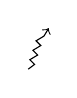
\begin{tikzpicture}[x=0.2cm,y=0.2cm]
\draw (0,0)--(0.4,0.3)--(0.1,0.6)--(0.6,0.9)--(0.3,1.2)--(0.8,1.5)--(0.5,1.8)--(1,2.1);
\draw[->] (1,2.1)--(1.3,2.6);
\end{tikzpicture}}}
\deleted{\unsure{on conclut}} et on conclut
\[
\begin{aligned}
&\overset{\text{chgt. de base}}{\simeq}
\mathbf L\Delta_B^*\bigl(\mathbf R\operatorname{pr}_{34*}\bigl(\operatorname{pr}_{13}'{}^*(F\otimes_S\mathcal L)\overset{\mathbf L}{\otimes}\operatorname{pr}_{24}'{}^*(G\otimes_S\mathcal L)\bigr)\bigr)\\
&\overset{\text{Künneth}}{\simeq}
\mathbf L\Delta_B^*\bigl(\mathbf R\operatorname{pr}_2(F\otimes\mathcal L)\overset{\mathbf L}{\otimes}_S\mathbf R\operatorname{pr}_{2*}(G\otimes\mathcal L)\bigr)\\
&\overset{\mathrm{déf}}{\simeq}
\mathbf L\Delta_B^*\bigl(\Phi(F)\overset{\mathbf L}{\otimes}_S\Phi(G)\bigr)\\
&\simeq\Phi(F)\overset{\mathbf L}{\otimes}\Phi(G).
\end{aligned}
\]
cqfd.

\deleted{\uline{Proposition!}} \inserted{\uline{Théorème}} Soient $A$, \deleted{deux} \inserted{$B$} schémas abéliens sur $S$, \inserted{de dim relative $n$,} \deleted{\unsure{B}} $\mathcal L$ un\\
Module inversible birigidifié sur $A\times B$, définissant une\\
\uline{dualité} entre $A$ et $B$. \deleted{Considérons} \inserted{Alors le composé} des deux
\diagram{\begin{tikzcd}[ampersand replacement=\&]
K(A) \arrow[r,dash,"\varphi_{\mathcal L}"] \& K(B) \arrow[r,dash,"\varphi_{{}^s\mathcal L}"] \& K(A)
\end{tikzcd}}
est \deleted{l'identité} \inserted{$(-1)^n\unsure{s_A^*|\sigma_A^*}$ (où $\unsure{s_A|\sigma_A}$ est la symétrie de $A$)} (donc, par symétrie, on voit que $\varphi_{\mathcal L}$ et $\inserted{\text{\textcircled{$(-1)^n$}}}\unsure{s_A^*|\sigma_A^*}\varphi_{{}^s\mathcal L}$\\
sont des isomorphismes inverses l'un de l'autre).
\mspage{3}
